\PassOptionsToPackage{unicode=true}{hyperref} % options for packages loaded elsewhere
\PassOptionsToPackage{hyphens}{url}
%
\documentclass[australian,ignorenonframetext,aspectratio=169]{beamer}
\usepackage{pgfpages}
\setbeamertemplate{caption}[numbered]
\setbeamertemplate{caption label separator}{: }
\setbeamercolor{caption name}{fg=normal text.fg}
\beamertemplatenavigationsymbolsempty
% Prevent slide breaks in the middle of a paragraph:
\widowpenalties 1 10000
\raggedbottom
\setbeamertemplate{part page}{
\centering
\begin{beamercolorbox}[sep=16pt,center]{part title}
  \usebeamerfont{part title}\insertpart\par
\end{beamercolorbox}
}
\setbeamertemplate{section page}{
\centering
\begin{beamercolorbox}[sep=12pt,center]{part title}
  \usebeamerfont{section title}\insertsection\par
\end{beamercolorbox}
}
\setbeamertemplate{subsection page}{
\centering
\begin{beamercolorbox}[sep=8pt,center]{part title}
  \usebeamerfont{subsection title}\insertsubsection\par
\end{beamercolorbox}
}
\AtBeginPart{
  \frame{\partpage}
}
\AtBeginSection{
  \ifbibliography
  \else
    \frame{\sectionpage}
  \fi
}
\AtBeginSubsection{
  \frame{\subsectionpage}
}
\usepackage{lmodern}
\usepackage{amssymb,amsmath}
\usepackage{ifxetex,ifluatex}
\usepackage{fixltx2e} % provides \textsubscript
\ifnum 0\ifxetex 1\fi\ifluatex 1\fi=0 % if pdftex
  \usepackage[T1]{fontenc}
  \usepackage[utf8]{inputenc}
  \usepackage{textcomp} % provides euro and other symbols
\else % if luatex or xelatex
  \usepackage{unicode-math}
  \defaultfontfeatures{Ligatures=TeX,Scale=MatchLowercase}
\fi
\usetheme[]{metropolis}
% use upquote if available, for straight quotes in verbatim environments
\IfFileExists{upquote.sty}{\usepackage{upquote}}{}
% use microtype if available
\IfFileExists{microtype.sty}{%
\usepackage[]{microtype}
\UseMicrotypeSet[protrusion]{basicmath} % disable protrusion for tt fonts
}{}
\IfFileExists{parskip.sty}{%
\usepackage{parskip}
}{% else
\setlength{\parindent}{0pt}
\setlength{\parskip}{6pt plus 2pt minus 1pt}
}
\usepackage{hyperref}
\hypersetup{
            pdftitle={Multiple regression with interaction terms},
            pdfauthor={Luis Castro-de-Araujo},
            pdfborder={0 0 0},
            breaklinks=true}
\urlstyle{same}  % don't use monospace font for urls
\newif\ifbibliography
\usepackage{color}
\usepackage{fancyvrb}
\newcommand{\VerbBar}{|}
\newcommand{\VERB}{\Verb[commandchars=\\\{\}]}
\DefineVerbatimEnvironment{Highlighting}{Verbatim}{commandchars=\\\{\}}
% Add ',fontsize=\small' for more characters per line
\usepackage{framed}
\definecolor{shadecolor}{RGB}{248,248,248}
\newenvironment{Shaded}{\begin{snugshade}}{\end{snugshade}}
\newcommand{\AlertTok}[1]{\textcolor[rgb]{0.94,0.16,0.16}{#1}}
\newcommand{\AnnotationTok}[1]{\textcolor[rgb]{0.56,0.35,0.01}{\textbf{\textit{#1}}}}
\newcommand{\AttributeTok}[1]{\textcolor[rgb]{0.77,0.63,0.00}{#1}}
\newcommand{\BaseNTok}[1]{\textcolor[rgb]{0.00,0.00,0.81}{#1}}
\newcommand{\BuiltInTok}[1]{#1}
\newcommand{\CharTok}[1]{\textcolor[rgb]{0.31,0.60,0.02}{#1}}
\newcommand{\CommentTok}[1]{\textcolor[rgb]{0.56,0.35,0.01}{\textit{#1}}}
\newcommand{\CommentVarTok}[1]{\textcolor[rgb]{0.56,0.35,0.01}{\textbf{\textit{#1}}}}
\newcommand{\ConstantTok}[1]{\textcolor[rgb]{0.00,0.00,0.00}{#1}}
\newcommand{\ControlFlowTok}[1]{\textcolor[rgb]{0.13,0.29,0.53}{\textbf{#1}}}
\newcommand{\DataTypeTok}[1]{\textcolor[rgb]{0.13,0.29,0.53}{#1}}
\newcommand{\DecValTok}[1]{\textcolor[rgb]{0.00,0.00,0.81}{#1}}
\newcommand{\DocumentationTok}[1]{\textcolor[rgb]{0.56,0.35,0.01}{\textbf{\textit{#1}}}}
\newcommand{\ErrorTok}[1]{\textcolor[rgb]{0.64,0.00,0.00}{\textbf{#1}}}
\newcommand{\ExtensionTok}[1]{#1}
\newcommand{\FloatTok}[1]{\textcolor[rgb]{0.00,0.00,0.81}{#1}}
\newcommand{\FunctionTok}[1]{\textcolor[rgb]{0.00,0.00,0.00}{#1}}
\newcommand{\ImportTok}[1]{#1}
\newcommand{\InformationTok}[1]{\textcolor[rgb]{0.56,0.35,0.01}{\textbf{\textit{#1}}}}
\newcommand{\KeywordTok}[1]{\textcolor[rgb]{0.13,0.29,0.53}{\textbf{#1}}}
\newcommand{\NormalTok}[1]{#1}
\newcommand{\OperatorTok}[1]{\textcolor[rgb]{0.81,0.36,0.00}{\textbf{#1}}}
\newcommand{\OtherTok}[1]{\textcolor[rgb]{0.56,0.35,0.01}{#1}}
\newcommand{\PreprocessorTok}[1]{\textcolor[rgb]{0.56,0.35,0.01}{\textit{#1}}}
\newcommand{\RegionMarkerTok}[1]{#1}
\newcommand{\SpecialCharTok}[1]{\textcolor[rgb]{0.00,0.00,0.00}{#1}}
\newcommand{\SpecialStringTok}[1]{\textcolor[rgb]{0.31,0.60,0.02}{#1}}
\newcommand{\StringTok}[1]{\textcolor[rgb]{0.31,0.60,0.02}{#1}}
\newcommand{\VariableTok}[1]{\textcolor[rgb]{0.00,0.00,0.00}{#1}}
\newcommand{\VerbatimStringTok}[1]{\textcolor[rgb]{0.31,0.60,0.02}{#1}}
\newcommand{\WarningTok}[1]{\textcolor[rgb]{0.56,0.35,0.01}{\textbf{\textit{#1}}}}
\usepackage{longtable,booktabs}
\usepackage{caption}
% These lines are needed to make table captions work with longtable:
\makeatletter
\def\fnum@table{\tablename~\thetable}
\makeatother
\usepackage{graphicx,grffile}
\makeatletter
\def\maxwidth{\ifdim\Gin@nat@width>\linewidth\linewidth\else\Gin@nat@width\fi}
\def\maxheight{\ifdim\Gin@nat@height>\textheight\textheight\else\Gin@nat@height\fi}
\makeatother
% Scale images if necessary, so that they will not overflow the page
% margins by default, and it is still possible to overwrite the defaults
% using explicit options in \includegraphics[width, height, ...]{}
\setkeys{Gin}{width=\maxwidth,height=\maxheight,keepaspectratio}
\setlength{\emergencystretch}{3em}  % prevent overfull lines
\providecommand{\tightlist}{%
  \setlength{\itemsep}{0pt}\setlength{\parskip}{0pt}}
\setcounter{secnumdepth}{0}

% set default figure placement to htbp
\makeatletter
\def\fps@figure{htbp}
\makeatother

\usepackage{navigator}
\embeddedfile{project}{2022-presentation.Rmd}
 \usepackage{appendixnumberbeamer}
 \usepackage{roboto}
\usepackage[font={footnotesize}]{caption}
\setbeamerfont{footnote}{size=\tiny}
\metroset{sectionpage=progressbar, titleformat=smallcaps}
\setbeamercolor{itemize item}{fg=vcuyellow}
\setbeamercolor{itemize subitem}{fg=vcuyellow}
\setbeamercolor{itemize subsubitem}{fg=vcuyellow}
 \setbeamertemplate{itemize item}[circle]
 \setbeamertemplate{itemize subitem}[square]
 \setbeamertemplate{itemize subsubitem}[triangle]
 \titlegraphic{%
 \hfill
\includegraphics[width=3cm,height=1.6cm,keepaspectratio]{style/VCU-Logo.png}}
 \definecolor{vcuyellow}{HTML}{FDBD10}
\setbeamercolor{palette primary}{fg=vcuyellow, bg=black}
 \setbeamercolor{frametitle}{fg=vcuyellow, bg=black}
 \setbeamercolor{titlelike}{fg=black}
 \setbeamercolor{titlepage}{fg=black, bg=vcuyellow}
 \setbeamercolor{footnote}{bg=black}
 \setbeamercolor{normal text}{fg=black}
 \setbeamercolor{block title}{fg=black, bg=vcuyellow!40!white}
 \setbeamercolor{alerted text}{fg=red}
 \setbeamercolor{example text}{fg=black}
 \setbeamercolor{title separator}{fg = vcuyellow, bg=vcuyellow}
\setbeamercolor{progress bar}{bg=white, fg=vcuyellow}
\setbeamercolor{progress bar in head/foot}{bg=white, fg=vcuyellow}
 \setbeamercolor{progress bar in section page}{bg=white, fg=vcuyellow}
\makeatletter
\newsavebox{\mybox}
\setbeamertemplate{frametitle}{%
 \nointerlineskip%
 \savebox{\mybox}{%
     \begin{beamercolorbox}[%
         wd=\paperwidth,%
         sep=0pt,%
         leftskip=\metropolis@frametitle@padding,%
         rightskip=\metropolis@frametitle@padding,%
       ]{frametitle}%
     \metropolis@frametitlestrut@start\insertframetitle\metropolis@frametitlestrut@end%
     \end{beamercolorbox}%
   }
 \begin{beamercolorbox}[%
     wd=\paperwidth,%
     sep=0pt,%
     leftskip=\metropolis@frametitle@padding,%
     rightskip=\metropolis@frametitle@padding,%
   ]{frametitle}%
 \metropolis@frametitlestrut@start\insertframetitle\metropolis@frametitlestrut@end%
 \hfill%
 \raisebox{-\metropolis@frametitle@padding}{
\includegraphics[height=\dimexpr\ht\mybox+\metropolis@frametitle@padding\relax]{style/VCU-Logo.png}}%
   \hspace*{-\metropolis@frametitle@padding}
 \end{beamercolorbox}%
}
\makeatother
 \makeatletter
 \pretocmd{\beamer@reseteecodes}{%
   \ifbool{metropolis@standout}{
     \endgroup
     \boolfalse{metropolis@standout}
   }{}
 }{}{}
 \makeatother
\ifnum 0\ifxetex 1\fi\ifluatex 1\fi=0 % if pdftex
  \usepackage[shorthands=off,main=australian]{babel}
\else
  % load polyglossia as late as possible as it *could* call bidi if RTL lang (e.g. Hebrew or Arabic)
  \usepackage{polyglossia}
  \setmainlanguage[variant=australian]{english}
\fi

\title{Multiple regression with interaction terms}
\author{Luis Castro-de-Araujo\footnote<.->{Post-doc T32.
  \href{mailto:luis.araujo@vcuhealth.org}{\nolinkurl{luis.araujo@vcuhealth.org}}\\}}
\providecommand{\institute}[1]{}
\institute{Virginia Institute for Psychiatric and Behavioral Genetics}
\date{11/07/2022}

\begin{document}
\frame{\titlepage}

\begin{frame}
\tableofcontents[hideallsubsections]
\end{frame}
\begin{frame}

\section{Multiple regression recap}

\end{frame}

\begin{frame}{Multiple Linear Regression}
\protect\hypertarget{multiple-linear-regression}{}

\begin{itemize}
\tightlist
\item
  Extension of the simple linear regression model to two or more
  independent variables
\end{itemize}

\[y = \beta_0 + \beta_1x_1 + \beta_2x_2 + \dots + \beta_px_p + \epsilon\]

\begin{itemize}
\item
  Expression = Baseline + Age + Tissue + Sex + Error
\item
  Partial Regression Coefficients: effect on the dependent variable when
  increasing the \emph{i}\textsuperscript{th} independent variable by 1
  unit, \textbf{holding all other predictors constant}
\end{itemize}

\end{frame}

\begin{frame}{Categorical Independent Variables}
\protect\hypertarget{categorical-independent-variables}{}

\begin{itemize}
\item
  Qualitative variables are easily incorporated in regression framework
  through \textbf{\emph{dummy variables}}
\item
  Simple example: sex can be coded as 0/1
\item
  What if my categorical variable contains three levels:
\end{itemize}

\[
\begin{aligned}
& \mathrm{x}_{1}=\left\{\begin{array}{l}0 \text { if } \mathrm{AA} 
                  \\1 \text { if } \mathrm{AG} 
                  \\2 \text { if } \mathrm{GG}\end{array}\right. 
\end{aligned}
\]

\end{frame}

\begin{frame}{Categorical Independent Variables}
\protect\hypertarget{categorical-independent-variables-1}{}

\begin{columns}[T]
\begin{column}{0.5\textwidth}
\begin{itemize}
\item
  Previous coding would result in \textbf{\emph{colinearity}}
\item
  Solution is to set up a series of dummy variable.
\item
  for k levels you need k-1 dummy variables
\end{itemize}

\[
\begin{aligned}
& \mathrm{x}_{1}=\left\{\begin{array}{l}1 \text { if } \mathrm{AA} \\0 \text { otherwise }\end{array}\right. \\
& x_{2}=\left\{\begin{array}{l}1 \text { if } A G \\0 \text { otherwise }\end{array}\right.
\end{aligned}
\]
\end{column}

\begin{column}{0.5\textwidth}
\begin{longtable}[]{@{}ccc@{}}
\toprule
& x1 & x2\tabularnewline
\midrule
\endhead
AA & 1 & 0\tabularnewline
AG & 0 & 1\tabularnewline
GG & 0 & 0\tabularnewline
\bottomrule
\end{longtable}
\end{column}
\end{columns}

\end{frame}

\begin{frame}{Assumptions}
\protect\hypertarget{assumptions}{}

\begin{description}
\tightlist
\item[Validity]
Does the data we're modeling matches the problem we're actually trying
to solve?
\item[Representativeness]
Is the sample data used in the regression model representative of the
population to which it will be applied?
\item[Additivity and Linearity]
The deterministic component of a regression model is a linear function
of the separate predictors: \(y=B_0 + B_1x_1 + ... + B_px_p\)
\item[Independence of Errors]
The errors from our model are independent.
\item[Homoscedasticity]
The errors from our model have equal variance.
\item[Normality of Errors]
The errors from our model are normally distributed.
\end{description}

\end{frame}

\begin{frame}{Multivariate regression}
\protect\hypertarget{multivariate-regression}{}

\begin{columns}[T]
\begin{column}{0.5\textwidth}
\begin{center}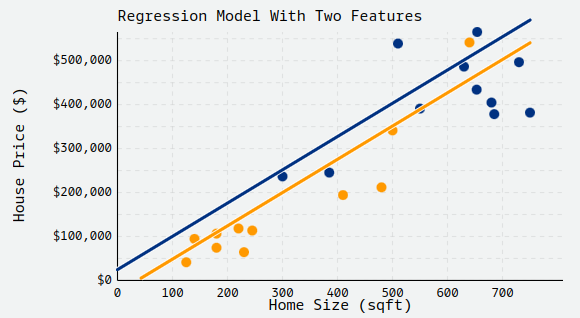
\includegraphics[width=1\linewidth]{../graphs/interpret-3} \end{center}

\tiny

\[house price=-27154+757*sqft+51867*pool\]

\begin{itemize}
\tightlist
\item
  In our example, we model home prices as a function of both the size of
  the house (sqft) and whether or not it has a pool
\end{itemize}
\end{column}

\begin{column}{0.5\textwidth}
\tiny

\begin{itemize}
\item
  intercept: -\$27,154, the predicted average housing price for houses
  with all x\textsubscript{i} = 0. Or the cost of houses with no pools
  and a square-footage of zero.
\item
  coefficient of pool: \$51,867, average expected price difference in
  houses of the same size (in sqft) if they do or do not have a pool. In
  other words, we expect, on average, houses of the same size to cost
  \$51,867 more if they have a pool than if they do not.
\item
  coefficient of sqft: \$757, average expected price difference in
  housing price for houses that have the same value of pool but differ
  in size by one square-foot.
\item
  We assume the same slope for sqft.Hence, two lines. This isn't always
  a valid assumption to make.
\end{itemize}
\end{column}
\end{columns}

\end{frame}

\begin{frame}{Back to our housing example, now with interactions}
\protect\hypertarget{back-to-our-housing-example-now-with-interactions}{}

\begin{columns}[T]
\begin{column}{0.5\textwidth}
\begin{center}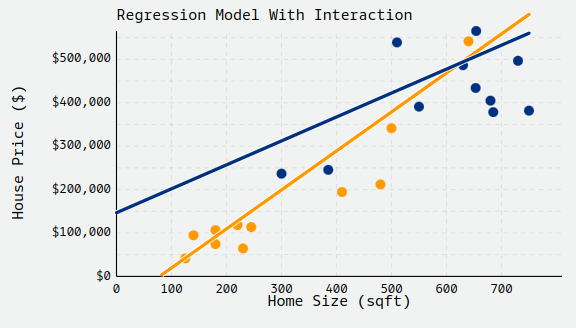
\includegraphics[width=1\linewidth]{../graphs/interpret-4} \end{center}

\tiny

\[house price=-70296+899*sqft+217111*pool-347*(sqft:pool)\]

\begin{itemize}
\tightlist
\item
  If we believe that the slope for sqft should differ between houses
  that do have pools and houses that do not, we can add an interaction
  term to our model, (sqft:pool).
\end{itemize}
\end{column}

\begin{column}{0.5\textwidth}
\tiny

\begin{itemize}
\item
  interaction term: -\$347, represents the difference in the slope for
  sqft, comparing houses that do and do not have pools. Visually, this
  represents the difference between the slopes of the two lines.
\item
  intercept: -\$70,296, represents the predicted housing price for
  houses with no pools and a square-footage of zero.
\item
  coefficient of pool: \$217,111, represents the average expected
  difference in houses of the same size (0 sqft) that differed in
  whether or not they had a pool. (It's not super useful since we don't
  have houses with 0 square-feet).
\item
  coefficient of sqft: \$899, represents the average expected difference
  in housing price for houses that do not have a pool (pool= 0) but
  differ in size by one square-foot.
\end{itemize}
\end{column}
\end{columns}

\end{frame}

\begin{frame}{}
\protect\hypertarget{section}{}

\section{Interaction terms}

\end{frame}

\begin{frame}{What is an Interaction?}
\protect\hypertarget{what-is-an-interaction}{}

\begin{itemize}
\tightlist
\item
  An interaction is a predictor that is some combination of the other
  predictors.
\end{itemize}

\end{frame}

\begin{frame}{Constructing an interaction}
\protect\hypertarget{constructing-an-interaction}{}

\begin{itemize}
\tightlist
\item
  Interactions are often the product of two or more predictors.
\item
  Can be written as,
\end{itemize}

\[Y = \beta_0 + \beta_1X_1 + \beta_2X_2 + \beta_3X_1X_2 + \epsilon\]

\end{frame}

\begin{frame}{Conditional vs.~marginal effects}
\protect\hypertarget{conditional-vs.-marginal-effects}{}

\begin{itemize}
\item
  Conditional effects: the effect of a predictor on the response,
  holding all other predictors constant.
\item
  Marginal effects: the effect of a predictor on the response, averaged
  over all values of the other predictors.
\end{itemize}

\end{frame}

\begin{frame}{Conditional vs.~marginal effects}
\protect\hypertarget{conditional-vs.-marginal-effects-1}{}

\begin{itemize}
\tightlist
\item
  If the conditional effects of X1 on Y at different levels of X2 are
  all the same then there is no interaction.
\end{itemize}

\end{frame}

\begin{frame}{Interpreting interaction effects}
\protect\hypertarget{interpreting-interaction-effects}{}

\small

\begin{longtable}[]{@{}lll@{}}
\toprule
\begin{minipage}[b]{0.09\columnwidth}\raggedright
Parameter\strut
\end{minipage} & \begin{minipage}[b]{0.28\columnwidth}\raggedright
Meaning\strut
\end{minipage} & \begin{minipage}[b]{0.55\columnwidth}\raggedright
Where people (used to) go awry\strut
\end{minipage}\tabularnewline
\midrule
\endhead
\begin{minipage}[t]{0.09\columnwidth}\raggedright
\(\beta_0\)\strut
\end{minipage} & \begin{minipage}[t]{0.28\columnwidth}\raggedright
Expected value of the DV when X1 and X2 ==0\strut
\end{minipage} & \begin{minipage}[t]{0.55\columnwidth}\raggedright
People get this\strut
\end{minipage}\tabularnewline
\begin{minipage}[t]{0.09\columnwidth}\raggedright
\(\beta_1\)\strut
\end{minipage} & \begin{minipage}[t]{0.28\columnwidth}\raggedright
Effect of X1 when X2 == 0\strut
\end{minipage} & \begin{minipage}[t]{0.55\columnwidth}\raggedright
Not marginal effects!\strut
\end{minipage}\tabularnewline
\begin{minipage}[t]{0.09\columnwidth}\raggedright
\(\beta_2\)\strut
\end{minipage} & \begin{minipage}[t]{0.28\columnwidth}\raggedright
Effect of X2 when X1 == 0\strut
\end{minipage} & \begin{minipage}[t]{0.55\columnwidth}\raggedright
Not marginal effects!\strut
\end{minipage}\tabularnewline
\begin{minipage}[t]{0.09\columnwidth}\raggedright
\(\beta_3\)\strut
\end{minipage} & \begin{minipage}[t]{0.28\columnwidth}\raggedright
The addition to the conditional effect when both X! and X2 are 1\strut
\end{minipage} & \begin{minipage}[t]{0.55\columnwidth}\raggedright
People just look at the significance of the interaction parameter and do
not calculate the underlying marginal or conditional effects or standard
errors\strut
\end{minipage}\tabularnewline
\bottomrule
\end{longtable}

\end{frame}

\begin{frame}[fragile]{In the past it was common to see standard errors
wrongly calculated}
\protect\hypertarget{in-the-past-it-was-common-to-see-standard-errors-wrongly-calculated}{}

\begin{itemize}
\tightlist
\item
  A common mistake that people make when interpreting interaction models
  is using the wrong standard errors.
\item
  The standard errors that are printed in every regression table are the
  positive square roots of the diagonal elements of the variance-
  covariance matrix of \(\beta\)
\item
  This does not matter anymore because of \texttt{margins()}
\end{itemize}

\end{frame}

\begin{frame}{Interaction and dummmy variable, Iris flower data set}
\protect\hypertarget{interaction-and-dummmy-variable-iris-flower-data-set}{}

\begin{columns}[T]
\begin{column}{0.5\textwidth}
\[\widehat{petal.length}_i = \beta_0 + \beta_1 sepal.length_i  \]
\end{column}

\begin{column}{0.5\textwidth}
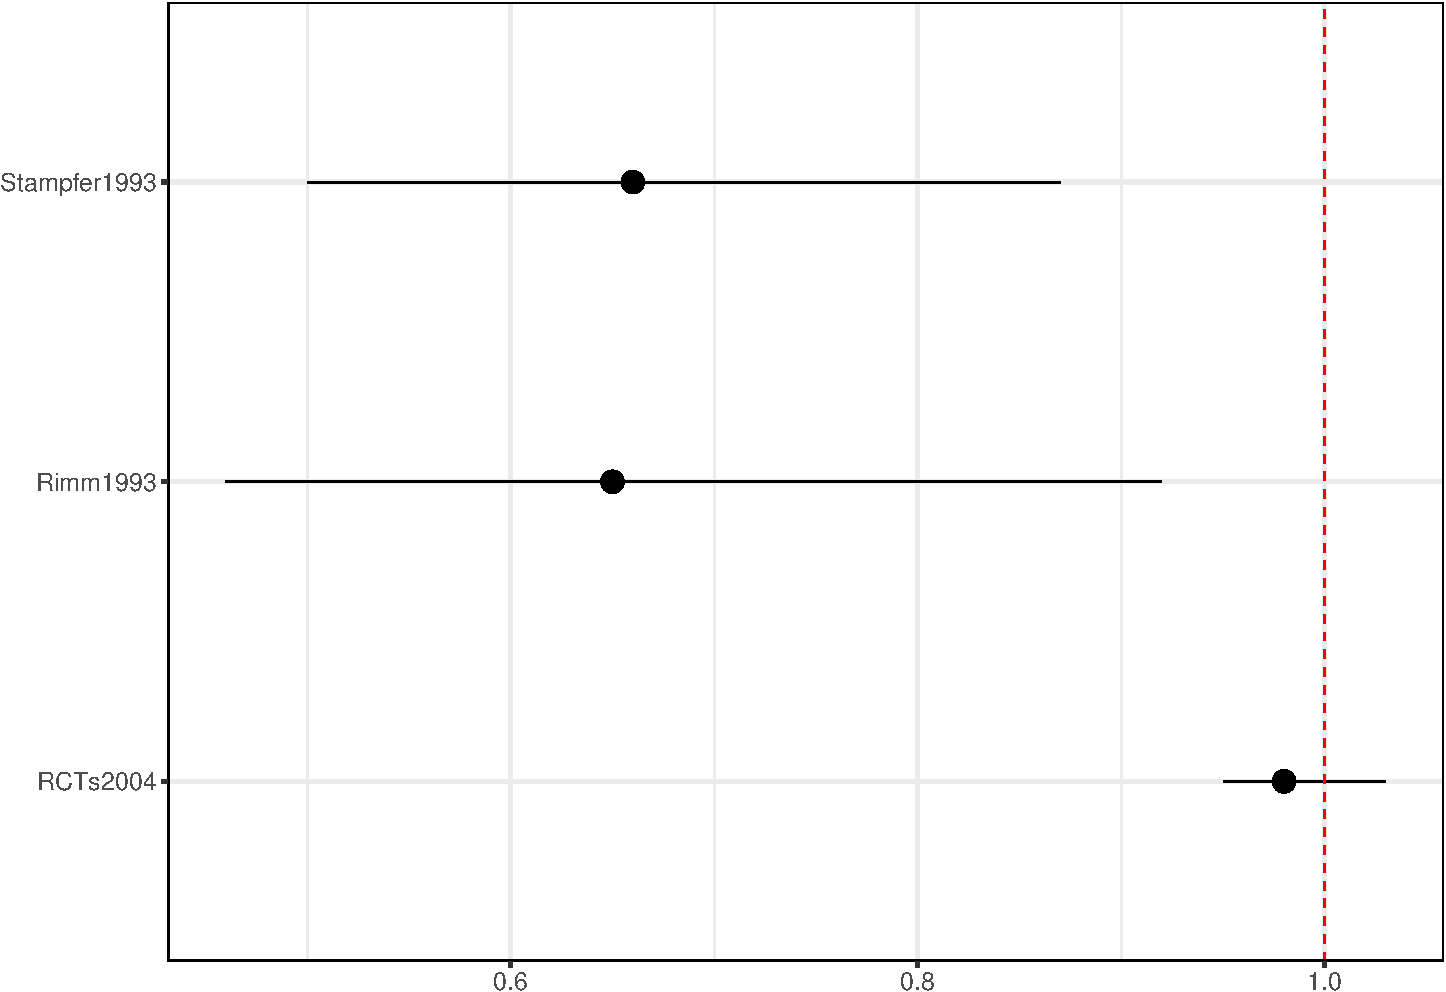
\includegraphics{../graphs/unnamed-chunk-3-1.pdf}
\end{column}
\end{columns}

\end{frame}

\begin{frame}{Let's improve the model?}
\protect\hypertarget{lets-improve-the-model}{}

\begin{block}{Creating the dummy}

\[\begin{aligned} \text { setosa }_i &=\left\{\begin{array}{l}1 \text { if species of flower } \mathrm{i}=\text { setosa }, \forall i \in[1,150] \\ 0 \text { otherwise }\end{array}\right.\\ \text { versicolor }_i &=\left\{\begin{array}{l}1 \text { if species of flower } \mathrm{i}=\text { versicolor, } \forall i \in[1,150] \\ 0 \text { otherwise }\end{array}\right.\end{aligned}\]

\end{block}

\begin{block}{Our formula is then}

\[\widehat{petal.length}_i = \beta_0 + \beta_1 sepal.length_i + \beta_2 \text { setosa }_i + \beta_3 \text { versicolor }_i\]

\end{block}

\end{frame}

\begin{frame}{By substitution we get three lines with same slope}
\protect\hypertarget{by-substitution-we-get-three-lines-with-same-slope}{}

\tiny

\begin{block}{If it is setosa}

\[
\begin{aligned}
\widehat{petal.length}_i &= \beta_0 + \beta_1 sepal.length_i + \beta_2 \text { setosa }_i + \beta_3 \text { versicolor }_i \\
&= \beta_0 + \beta_1 sepal.length_i + \beta_2 1 + \beta_3 0 \\
&= \beta_0 + \beta_1 sepal.length_i + \beta_2 \\
&= (\beta_0 + \beta_2) + \beta_1 sepal.length_i
\end{aligned}
\]

\end{block}

\begin{block}{If it is versicolor}

\[
\begin{aligned}
\widehat{petal.length}_i &= \beta_0 + \beta_1 sepal.length_i + \beta_2 \text { setosa }_i + \beta_3 \text { versicolor }_i \\
&= \beta_0 + \beta_1 sepal.length_i + \beta_2 0 + \beta_3 1 \\
&= \beta_0 + \beta_1 sepal.length_i + \beta_3 \\
&= (\beta_0 + \beta_3) + \beta_1 sepal.length_i
\end{aligned}
\]

\end{block}

\begin{block}{If it is virginica}

\[
\begin{aligned}
\widehat{petal.length}_i &= \beta_0 + \beta_1 sepal.length_i + \beta_2 \text { setosa }_i + \beta_3 \text { versicolor }_i \\
&= \beta_0 + \beta_1 sepal.length_i + \beta_2 0 + \beta_3 0 \\
&= \beta_0 + \beta_1 sepal.length_i \\
&= \beta_0 + \beta_1 sepal.length_i
\end{aligned}
\]

\end{block}

\end{frame}

\begin{frame}[fragile]{Same slope, different intercepts}
\protect\hypertarget{same-slope-different-intercepts}{}

\begin{columns}[T]
\begin{column}{0.5\textwidth}
\tiny

\begin{Shaded}
\begin{Highlighting}[]
\NormalTok{iris}\OperatorTok{$}\NormalTok{pred \textless{}{-}}\StringTok{ }\KeywordTok{predict}\NormalTok{(}\KeywordTok{lm}\NormalTok{(Petal.Length }\OperatorTok{\textasciitilde{}}\StringTok{ }\NormalTok{Species}\OperatorTok{+}\NormalTok{Sepal.Length, }
                        \DataTypeTok{data =}\NormalTok{ iris))}

\CommentTok{\# plot in ggplot}
\KeywordTok{ggplot}\NormalTok{(iris, }\KeywordTok{aes}\NormalTok{(}\DataTypeTok{x =}\NormalTok{ Sepal.Length, }\DataTypeTok{y =}\NormalTok{ Petal.Length, }\DataTypeTok{color =}\NormalTok{ Species)) }\OperatorTok{+}
\StringTok{  }\KeywordTok{geom\_point}\NormalTok{() }\OperatorTok{+}\StringTok{ }
\StringTok{  }\KeywordTok{geom\_line}\NormalTok{(}\KeywordTok{aes}\NormalTok{(Sepal.Length, pred )) }\OperatorTok{+}
\StringTok{  }\KeywordTok{theme\_luis}\NormalTok{() }\OperatorTok{+}
\StringTok{  }\KeywordTok{theme}\NormalTok{( }\DataTypeTok{legend.position =} \KeywordTok{c}\NormalTok{(}\FloatTok{0.9}\NormalTok{, }\FloatTok{0.15}\NormalTok{))}
\end{Highlighting}
\end{Shaded}
\end{column}

\begin{column}{0.5\textwidth}
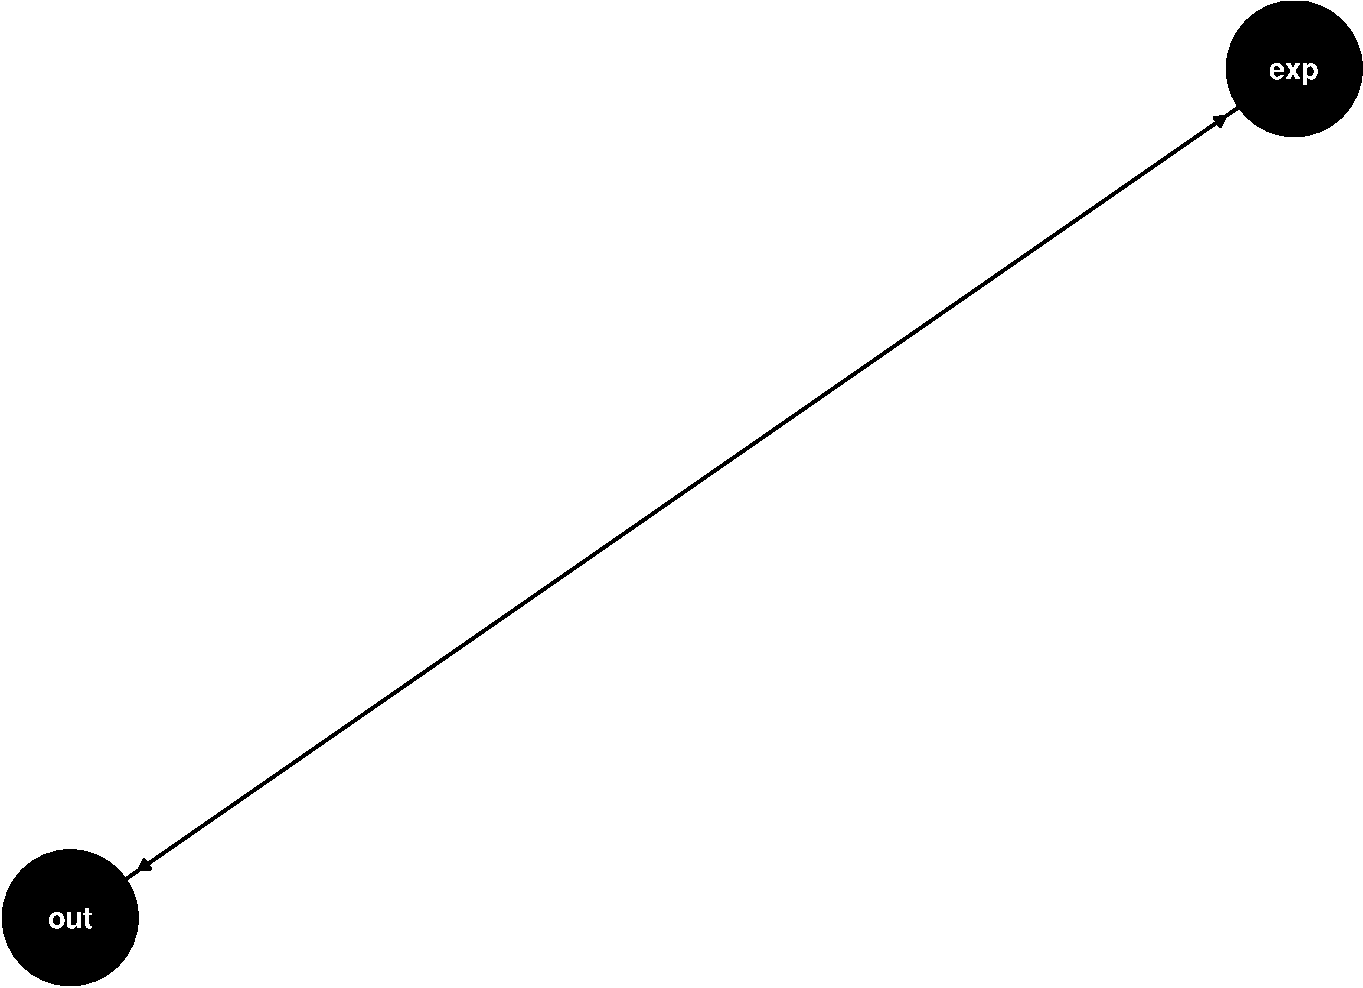
\includegraphics[width=1\linewidth]{../graphs/unnamed-chunk-5-1}
\end{column}
\end{columns}

\end{frame}

\begin{frame}[fragile]{Now we can add an interaction}
\protect\hypertarget{now-we-can-add-an-interaction}{}

\tiny

\[
\begin{aligned}
&\widehat{petal.length}_i = \beta_0 + \beta_1 sepal.length_i + \beta_2 \text { setosa }_i + \beta_3 \text { versicolor }_i \\
&+ \beta_4 sepal.length_i \text { setosa }_i + \beta_5 sepal.length_i \text { versicolor }_i
\end{aligned}
\]

\begin{itemize}
\tightlist
\item
  this will result in three unique lines depending on the species of the
  flower.
\item
  both the intercepts and the slopes will be allowed to be different.
\end{itemize}

\begin{block}{Does it make sense to retain the interaction?}

\tiny

\begin{verbatim}
# A tibble: 6 x 5
  term                           estimate std.error statistic    p.value
  <chr>                             <dbl>     <dbl>     <dbl>      <dbl>
1 (Intercept)                       0.803     0.531     1.51  0.133     
2 Sepal.Length                      0.132     0.106     1.24  0.216     
3 Speciesversicolor                -0.618     0.684    -0.904 0.368     
4 Speciesvirginica                 -0.193     0.658    -0.293 0.770     
5 Sepal.Length:Speciesversicolor    0.555     0.128     4.33  0.0000278 
6 Sepal.Length:Speciesvirginica     0.618     0.121     5.11  0.00000100
\end{verbatim}

\end{block}

\end{frame}

\begin{frame}[fragile]{Does it make sense to retain the interaction?}
\protect\hypertarget{does-it-make-sense-to-retain-the-interaction-1}{}

\tiny

\begin{Shaded}
\begin{Highlighting}[]
\NormalTok{broom}\OperatorTok{::}\KeywordTok{tidy}\NormalTok{(inter) }\OperatorTok{|}\ErrorTok{\textgreater{}}\StringTok{ }\KeywordTok{kable}\NormalTok{()}
\end{Highlighting}
\end{Shaded}

\begin{longtable}[]{@{}lrrrr@{}}
\toprule
term & estimate & std.error & statistic & p.value\tabularnewline
\midrule
\endhead
(Intercept) & 0.803 & 0.531 & 1.512 & 0.133\tabularnewline
Sepal.Length & 0.132 & 0.106 & 1.244 & 0.216\tabularnewline
Speciesversicolor & -0.618 & 0.684 & -0.904 & 0.368\tabularnewline
Speciesvirginica & -0.193 & 0.658 & -0.293 & 0.770\tabularnewline
Sepal.Length:Speciesversicolor & 0.555 & 0.128 & 4.330 &
0.000\tabularnewline
Sepal.Length:Speciesvirginica & 0.618 & 0.121 & 5.111 &
0.000\tabularnewline
\bottomrule
\end{longtable}

\begin{Shaded}
\begin{Highlighting}[]
\KeywordTok{anova}\NormalTok{(nospecies, w\_species, inter)}
\end{Highlighting}
\end{Shaded}

\begin{verbatim}
Analysis of Variance Table

Model 1: Petal.Length ~ Sepal.Length
Model 2: Petal.Length ~ Sepal.Length + Species
Model 3: Petal.Length ~ Sepal.Length + Species + Sepal.Length:Species
  Res.Df   RSS Df Sum of Sq     F               Pr(>F)    
1    148 111.5                                            
2    146  11.7  2      99.8 731.9 < 0.0000000000000002 ***
3    144   9.8  2       1.8  13.5            0.0000043 ***
---
Signif. codes:  0 '***' 0.001 '**' 0.01 '*' 0.05 '.' 0.1 ' ' 1
\end{verbatim}

\end{frame}

\begin{frame}[fragile]{Now we can add an interaction}
\protect\hypertarget{now-we-can-add-an-interaction-1}{}

\begin{columns}[T]
\begin{column}{0.5\textwidth}
\tiny

\[
\begin{aligned}
&\widehat{petal.length}_i = \beta_0 + \beta_1 sepal.length_i + \beta_2 \text { setosa }_i + \beta_3 \text { versicolor }_i \\
&+ \beta_4 sepal.length_i \text { setosa }_i + \beta_5 sepal.length_i \text { versicolor }_i
\end{aligned}
\]

\begin{itemize}
\tightlist
\item
  this will result in three unique lines depending on the species of the
  flower.
\item
  both the intercepts and the slopes will be allowed to be different.
\item
  ggplot geom\_smooth does this by default if \texttt{color} is used
\end{itemize}
\end{column}

\begin{column}{0.5\textwidth}
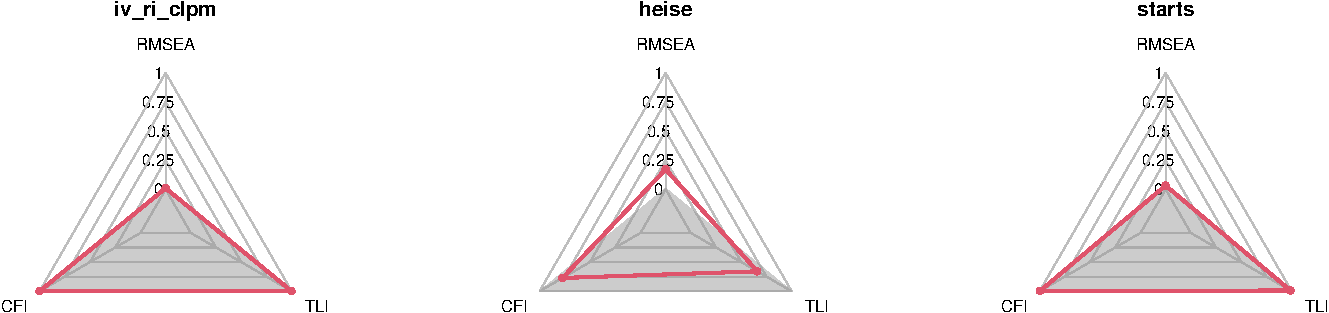
\includegraphics{../graphs/unnamed-chunk-8-1.pdf}
\end{column}
\end{columns}

\end{frame}

\begin{frame}[fragile]{Now we can add an interaction}
\protect\hypertarget{now-we-can-add-an-interaction-2}{}

\begin{columns}[T]
\begin{column}{0.5\textwidth}
\tiny

\begin{Shaded}
\begin{Highlighting}[]
\KeywordTok{ggplot}\NormalTok{(iris, }\KeywordTok{aes}\NormalTok{(}\DataTypeTok{x =}\NormalTok{ Sepal.Length, }\DataTypeTok{y =}\NormalTok{ Petal.Length, }\DataTypeTok{color =}\NormalTok{ Species)) }\OperatorTok{+}
\StringTok{  }\KeywordTok{geom\_point}\NormalTok{() }\OperatorTok{+}\StringTok{ }
\StringTok{  }\KeywordTok{geom\_smooth}\NormalTok{(}\DataTypeTok{method =} \StringTok{"lm"}\NormalTok{, }\DataTypeTok{se =} \OtherTok{FALSE}\NormalTok{) }\OperatorTok{+}
\StringTok{  }\KeywordTok{theme\_luis}\NormalTok{()}\OperatorTok{+}
\StringTok{  }\KeywordTok{theme}\NormalTok{( }\DataTypeTok{legend.position =} \KeywordTok{c}\NormalTok{(}\FloatTok{0.9}\NormalTok{, }\FloatTok{0.15}\NormalTok{))}
\end{Highlighting}
\end{Shaded}
\end{column}

\begin{column}{0.5\textwidth}

\includegraphics{../graphs/unnamed-chunk-10-1.pdf}
\end{column}
\end{columns}

\end{frame}

\begin{frame}{}
\protect\hypertarget{section-1}{}

\section{Visualizing interactions}

\end{frame}

\begin{frame}[fragile]{Mtcars data set - regression of speed on wt*cyl}
\protect\hypertarget{mtcars-data-set---regression-of-speed-on-wtcyl}{}

\begin{columns}[T]
\begin{column}{0.5\textwidth}
\tiny

\begin{Shaded}
\begin{Highlighting}[]
\NormalTok{fit \textless{}{-}}\StringTok{ }\KeywordTok{glm}\NormalTok{(qsec }\OperatorTok{\textasciitilde{}}\StringTok{ }\NormalTok{wt}\OperatorTok{*}\KeywordTok{as.factor}\NormalTok{(cyl), }\DataTypeTok{data =}\NormalTok{ mtcars)}
\KeywordTok{summary}\NormalTok{(fit)}
\end{Highlighting}
\end{Shaded}

\begin{itemize}
\tightlist
\item
  Note: not significant, but we will return to this later
  \texttt{summary(margins(fit))}
\end{itemize}
\end{column}

\begin{column}{0.5\textwidth}
\tiny

\begin{verbatim}

Call:
glm(formula = qsec ~ wt * as.factor(cyl), data = mtcars)

Deviance Residuals: 
   Min      1Q  Median      3Q     Max  
-2.163  -0.796   0.280   0.665   2.134  

Coefficients:
                   Estimate Std. Error t value      Pr(>|t|)    
(Intercept)          14.829      1.500    9.88 0.00000000027 ***
wt                    1.885      0.639    2.95        0.0066 ** 
as.factor(cyl)6      -9.782      4.395   -2.23        0.0349 *  
as.factor(cyl)8      -1.437      2.273   -0.63        0.5329    
wt:as.factor(cyl)6    2.263      1.464    1.55        0.1343    
wt:as.factor(cyl)8   -1.040      0.764   -1.36        0.1855    
---
Signif. codes:  0 '***' 0.001 '**' 0.01 '*' 0.05 '.' 0.1 ' ' 1

(Dispersion parameter for gaussian family taken to be 1.32)

    Null deviance: 98.988  on 31  degrees of freedom
Residual deviance: 34.398  on 26  degrees of freedom
AIC: 107.1

Number of Fisher Scoring iterations: 2
\end{verbatim}
\end{column}
\end{columns}

\end{frame}

\begin{frame}[fragile]{Regression of mpg on wt*cyl}
\protect\hypertarget{regression-of-mpg-on-wtcyl}{}

\begin{columns}[T]
\begin{column}{0.5\textwidth}
\tiny

\begin{Shaded}
\begin{Highlighting}[]
\NormalTok{fit \textless{}{-}}\StringTok{ }\KeywordTok{glm}\NormalTok{(mpg }\OperatorTok{\textasciitilde{}}\StringTok{ }\NormalTok{wt}\OperatorTok{*}\KeywordTok{as.factor}\NormalTok{(cyl), }\DataTypeTok{data =}\NormalTok{ mtcars)}
\KeywordTok{summary}\NormalTok{(fit)}
\end{Highlighting}
\end{Shaded}
\end{column}

\begin{column}{0.5\textwidth}
\tiny

\begin{verbatim}

Call:
glm(formula = mpg ~ wt * as.factor(cyl), data = mtcars)

Deviance Residuals: 
   Min      1Q  Median      3Q     Max  
-4.151  -1.380  -0.639   1.494   5.252  

Coefficients:
                   Estimate Std. Error t value        Pr(>|t|)    
(Intercept)           39.57       3.19   12.39 0.0000000000021 ***
wt                    -5.65       1.36   -4.15         0.00031 ***
as.factor(cyl)6      -11.16       9.36   -1.19         0.24358    
as.factor(cyl)8      -15.70       4.84   -3.24         0.00322 ** 
wt:as.factor(cyl)6     2.87       3.12    0.92         0.36620    
wt:as.factor(cyl)8     3.45       1.63    2.12         0.04344 *  
---
Signif. codes:  0 '***' 0.001 '**' 0.01 '*' 0.05 '.' 0.1 ' ' 1

(Dispersion parameter for gaussian family taken to be 6)

    Null deviance: 1126.05  on 31  degrees of freedom
Residual deviance:  155.89  on 26  degrees of freedom
AIC: 155.5

Number of Fisher Scoring iterations: 2
\end{verbatim}
\end{column}
\end{columns}

\end{frame}

\begin{frame}[fragile]{Regression of mpg on wt*cyl}
\protect\hypertarget{regression-of-mpg-on-wtcyl-1}{}

\begin{columns}[T]
\begin{column}{0.5\textwidth}
\tiny

\begin{Shaded}
\begin{Highlighting}[]
\NormalTok{pred \textless{}{-}}\StringTok{ }\KeywordTok{ggpredict}\NormalTok{(fit, }\DataTypeTok{terms =} \KeywordTok{c}\NormalTok{(}\StringTok{"wt"}\NormalTok{, }\StringTok{"cyl"}\NormalTok{))}
\KeywordTok{plot}\NormalTok{(pred, }\DataTypeTok{add.data =} \OtherTok{TRUE}\NormalTok{)}\OperatorTok{+}
\StringTok{  }\KeywordTok{theme\_luis}\NormalTok{()}\OperatorTok{+}
\StringTok{  }\KeywordTok{theme}\NormalTok{( }\DataTypeTok{legend.position =} \KeywordTok{c}\NormalTok{(}\FloatTok{0.1}\NormalTok{, }\FloatTok{0.15}\NormalTok{))}
\end{Highlighting}
\end{Shaded}
\end{column}

\begin{column}{0.5\textwidth}

\includegraphics{../graphs/unnamed-chunk-16-1.pdf}
\end{column}
\end{columns}

\end{frame}

\begin{frame}[fragile]{An interaction may not be sig across the entire
range of the predictor}
\protect\hypertarget{an-interaction-may-not-be-sig-across-the-entire-range-of-the-predictor}{}

\begin{columns}[T]
\begin{column}{0.5\textwidth}
\begin{block}{Let's see mpg \textasciitilde{} hp + wt}

\tiny

\begin{Shaded}
\begin{Highlighting}[]
\NormalTok{fit \textless{}{-}}\StringTok{ }\KeywordTok{glm}\NormalTok{(mpg }\OperatorTok{\textasciitilde{}}\StringTok{ }\NormalTok{hp}\OperatorTok{*}\NormalTok{wt, }\DataTypeTok{data =}\NormalTok{ mtcars)}
\NormalTok{pred \textless{}{-}}\StringTok{ }\KeywordTok{ggpredict}\NormalTok{(fit, }\DataTypeTok{terms =} \KeywordTok{c}\NormalTok{(}\StringTok{"hp"}\NormalTok{, }\StringTok{"wt"}\NormalTok{))}

\KeywordTok{plot}\NormalTok{(pred, }\DataTypeTok{add.data =} \OtherTok{TRUE}\NormalTok{) }\OperatorTok{+}
\StringTok{  }\KeywordTok{theme\_luis}\NormalTok{()}
\end{Highlighting}
\end{Shaded}

\end{block}
\end{column}

\begin{column}{0.5\textwidth}
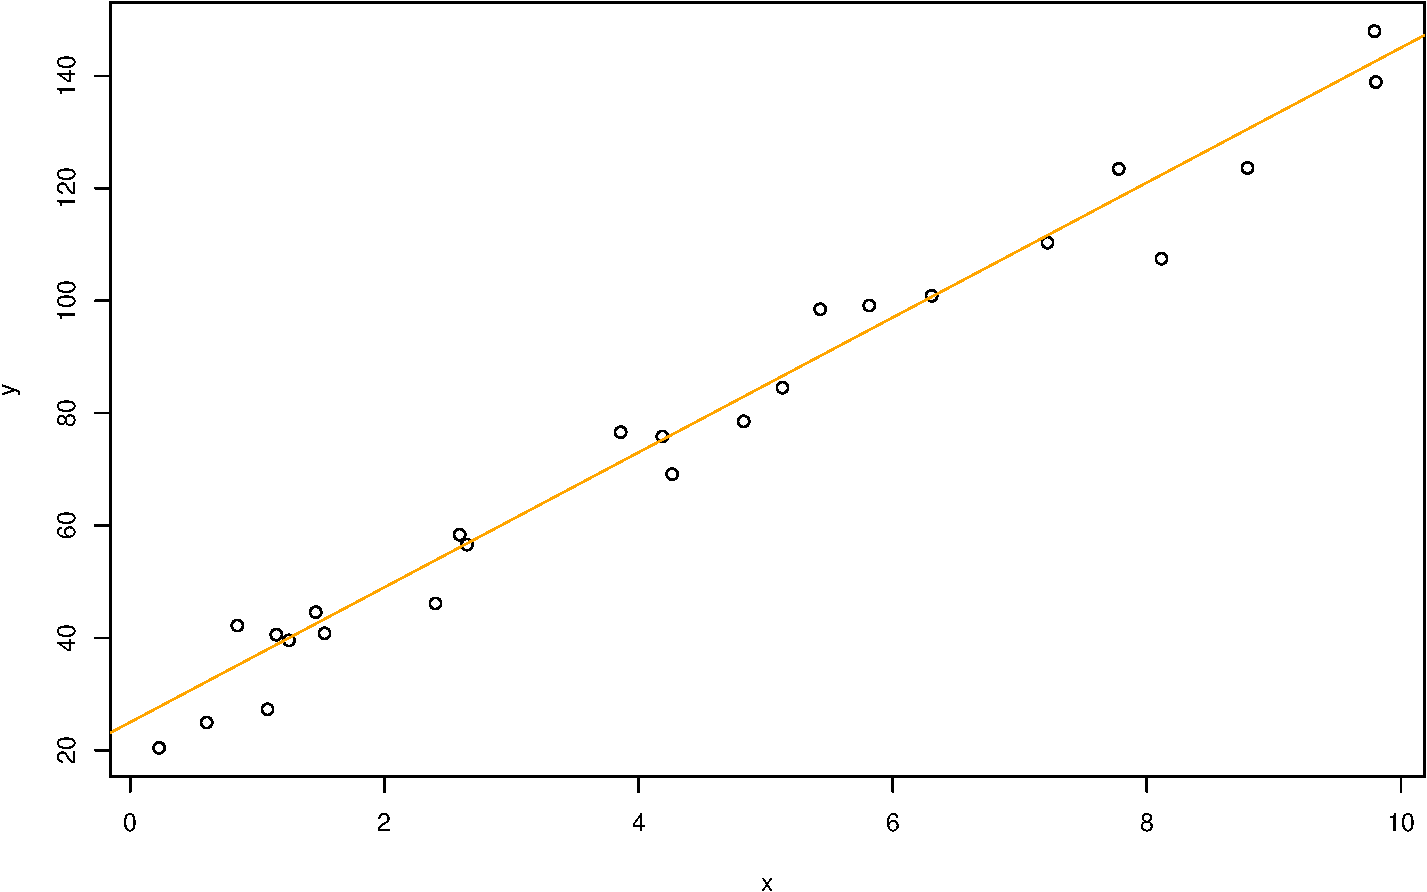
\includegraphics{../graphs/unnamed-chunk-18-1.pdf}
\end{column}
\end{columns}

\end{frame}

\begin{frame}[fragile]{Now, from what point the slope becomes non
signficant?}
\protect\hypertarget{now-from-what-point-the-slope-becomes-non-signficant}{}

\begin{columns}[T]
\begin{column}{0.5\textwidth}
\begin{block}{JOHNSON-NEYMAN INTERVAL}

\tiny

\begin{Shaded}
\begin{Highlighting}[]
\NormalTok{jn \textless{}{-}}\StringTok{ }\KeywordTok{johnson\_neyman}\NormalTok{(fit, wt, hp , }\DataTypeTok{plot =} \OtherTok{TRUE}\NormalTok{)}
\NormalTok{jn}
\end{Highlighting}
\end{Shaded}

\end{block}
\end{column}

\begin{column}{0.5\textwidth}
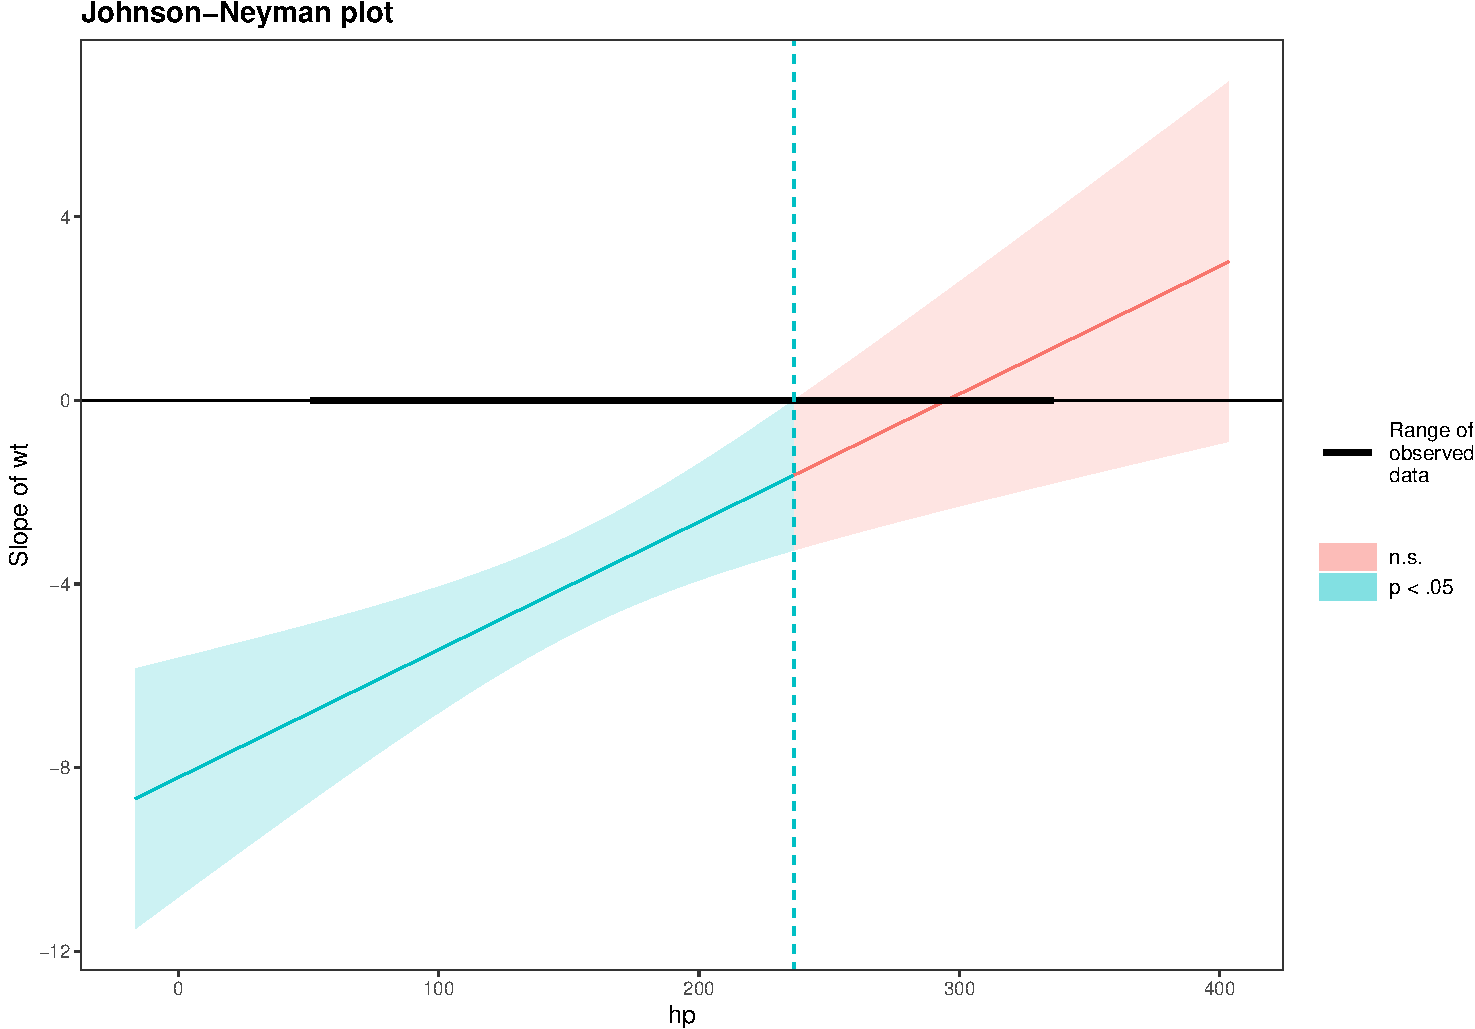
\includegraphics{../graphs/unnamed-chunk-20-1.pdf}
\end{column}
\end{columns}

\end{frame}

\begin{frame}[fragile]{Now, from what point the slope becomes non
signficant?}
\protect\hypertarget{now-from-what-point-the-slope-becomes-non-signficant-1}{}

\begin{columns}[T]
\begin{column}{0.5\textwidth}
\begin{block}{JOHNSON-NEYMAN INTERVAL - Overlayed over data}

\tiny

\begin{Shaded}
\begin{Highlighting}[]
\NormalTok{fit \textless{}{-}}\StringTok{ }\KeywordTok{glm}\NormalTok{(mpg }\OperatorTok{\textasciitilde{}}\StringTok{ }\NormalTok{hp}\OperatorTok{*}\NormalTok{wt, }\DataTypeTok{data =}\NormalTok{ mtcars)}
\NormalTok{pred \textless{}{-}}\StringTok{ }\KeywordTok{ggpredict}\NormalTok{(fit, }\DataTypeTok{terms =} \KeywordTok{c}\NormalTok{(}\StringTok{"hp"}\NormalTok{, }\StringTok{"wt"}\NormalTok{))}
\NormalTok{jn\textless{}{-}}\KeywordTok{johnson\_neyman}\NormalTok{(fit, wt, hp , }\DataTypeTok{plot =} \OtherTok{TRUE}\NormalTok{)}
\NormalTok{jn\_bound\textless{}{-}}\KeywordTok{as.numeric}\NormalTok{(jn}\OperatorTok{$}\NormalTok{bounds[}\DecValTok{1}\NormalTok{])  }

\KeywordTok{plot}\NormalTok{(pred, }\DataTypeTok{add.data=}\NormalTok{T) }\OperatorTok{+}\StringTok{ }
\StringTok{  }\KeywordTok{geom\_vline}\NormalTok{(}\DataTypeTok{xintercept =}\NormalTok{ jn\_bound, }\DataTypeTok{linetype =} \StringTok{"dashed"}\NormalTok{, }
             \DataTypeTok{color =} \StringTok{"red"}\NormalTok{)}\OperatorTok{+}
\StringTok{  }\KeywordTok{theme\_luis}\NormalTok{()}
\end{Highlighting}
\end{Shaded}

\end{block}
\end{column}

\begin{column}{0.5\textwidth}
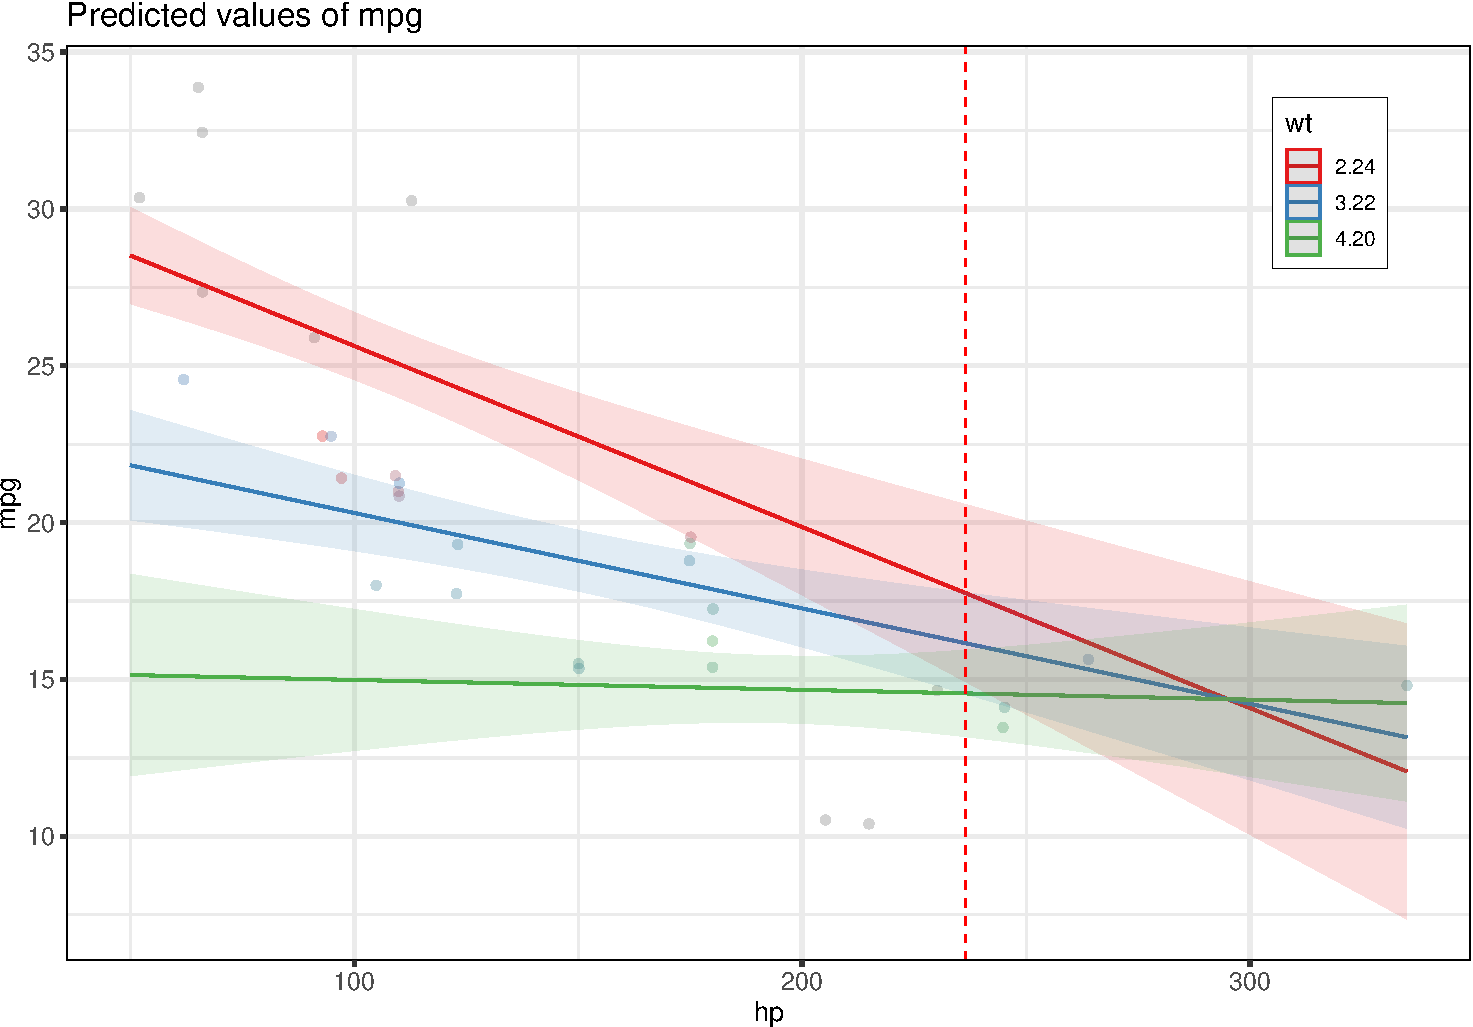
\includegraphics{../graphs/unnamed-chunk-22-1.pdf}
\end{column}
\end{columns}

\end{frame}

\begin{frame}[fragile]{Three-way interactions}
\protect\hypertarget{three-way-interactions}{}

\begin{columns}[T]
\begin{column}{0.5\textwidth}
\tiny

\begin{Shaded}
\begin{Highlighting}[]
\NormalTok{fit \textless{}{-}}\StringTok{ }\KeywordTok{glm}\NormalTok{(mpg }\OperatorTok{\textasciitilde{}}\StringTok{ }\NormalTok{hp}\OperatorTok{*}\NormalTok{wt}\OperatorTok{*}\NormalTok{cyl, }\DataTypeTok{data =}\NormalTok{ mtcars)}
\end{Highlighting}
\end{Shaded}

\begin{Shaded}
\begin{Highlighting}[]
\NormalTok{dat \textless{}{-}}\StringTok{ }\KeywordTok{ggpredict}\NormalTok{(fit, }\DataTypeTok{terms =} \KeywordTok{c}\NormalTok{(}\StringTok{"hp"}\NormalTok{, }\StringTok{"wt"}\NormalTok{, }\StringTok{"cyl"}\NormalTok{))}
\KeywordTok{plot}\NormalTok{(dat, }\DataTypeTok{ci =} \OtherTok{FALSE}\NormalTok{)}
\end{Highlighting}
\end{Shaded}

\tiny

\begin{verbatim}

Call:
glm(formula = mpg ~ hp * wt * cyl, data = mtcars)

Deviance Residuals: 
   Min      1Q  Median      3Q     Max  
-3.352  -1.464  -0.169   1.345   4.001  

Coefficients:
            Estimate Std. Error t value Pr(>|t|)
(Intercept) 43.96543   30.32070    1.45     0.16
hp          -0.02587    0.24000   -0.11     0.92
wt          -2.25515   10.68401   -0.21     0.83
cyl         -0.52189    6.33725   -0.08     0.94
hp:wt       -0.03666    0.09360   -0.39     0.70
hp:cyl      -0.00569    0.03850   -0.15     0.88
wt:cyl      -0.42991    1.99058   -0.22     0.83
hp:wt:cyl    0.00654    0.01375    0.48     0.64

(Dispersion parameter for gaussian family taken to be 4.88)

    Null deviance: 1126.05  on 31  degrees of freedom
Residual deviance:  117.18  on 24  degrees of freedom
AIC: 150.3

Number of Fisher Scoring iterations: 2
\end{verbatim}
\end{column}

\begin{column}{0.5\textwidth}
\begin{center}
\includegraphics{../graphs/unnamed-chunk-26-1} \end{center}
\end{column}
\end{columns}

\section{Marginal effects}

\end{frame}

\begin{frame}{Marginal effects}
\protect\hypertarget{marginal-effects}{}

\begin{itemize}
\tightlist
\item
  Marginal effects: the effect of a predictor on the response, averaged
  over all values of the other predictors.
\item
  It is achieved by..
\end{itemize}

\end{frame}

\begin{frame}[fragile]{What are the marginal effects of the latest
model?}
\protect\hypertarget{what-are-the-marginal-effects-of-the-latest-model}{}

\begin{Shaded}
\begin{Highlighting}[]
\NormalTok{fit\_m \textless{}{-}}\StringTok{ }\KeywordTok{margins}\NormalTok{(fit)}
\KeywordTok{summary}\NormalTok{(fit\_m)}
\end{Highlighting}
\end{Shaded}

\begin{verbatim}
 factor     AME     SE       z      p   lower   upper
    cyl  0.6261 1.3513  0.4633 0.6431 -2.0224  3.2745
     hp -0.0402 0.0152 -2.6390 0.0083 -0.0700 -0.0103
     wt -3.7134 0.7952 -4.6696 0.0000 -5.2720 -2.1547
\end{verbatim}

\end{frame}

\begin{frame}[fragile]{Plotting the marginal effects}
\protect\hypertarget{plotting-the-marginal-effects}{}

\begin{columns}[T]
\begin{column}{0.5\textwidth}
\tiny

\begin{Shaded}
\begin{Highlighting}[]
\NormalTok{fit\_mo \textless{}{-}}\StringTok{ }\KeywordTok{as\_tibble}\NormalTok{(}\KeywordTok{summary}\NormalTok{(fit\_m))}
\NormalTok{p \textless{}{-}}\StringTok{ }\KeywordTok{ggplot}\NormalTok{(}\DataTypeTok{data =}\NormalTok{ fit\_mo, }\KeywordTok{aes}\NormalTok{(}\DataTypeTok{x =} \KeywordTok{reorder}\NormalTok{(factor, AME),}
                              \DataTypeTok{y =}\NormalTok{ AME, }\DataTypeTok{ymin =}\NormalTok{ lower, }\DataTypeTok{ymax =}\NormalTok{ upper))}

\NormalTok{p }\OperatorTok{+}\StringTok{ }\KeywordTok{geom\_hline}\NormalTok{(}\DataTypeTok{yintercept =} \DecValTok{0}\NormalTok{, }\DataTypeTok{color =} \StringTok{"gray80"}\NormalTok{) }\OperatorTok{+}
\StringTok{    }\KeywordTok{geom\_pointrange}\NormalTok{() }\OperatorTok{+}\StringTok{ }\KeywordTok{coord\_flip}\NormalTok{() }\OperatorTok{+}
\StringTok{    }\KeywordTok{labs}\NormalTok{(}\DataTypeTok{x =} \OtherTok{NULL}\NormalTok{, }\DataTypeTok{y =} \StringTok{"Average Marginal Effect"}\NormalTok{) }\OperatorTok{+}\StringTok{ }
\StringTok{    }\KeywordTok{theme\_luis}\NormalTok{()}
\end{Highlighting}
\end{Shaded}
\end{column}

\begin{column}{0.5\textwidth}
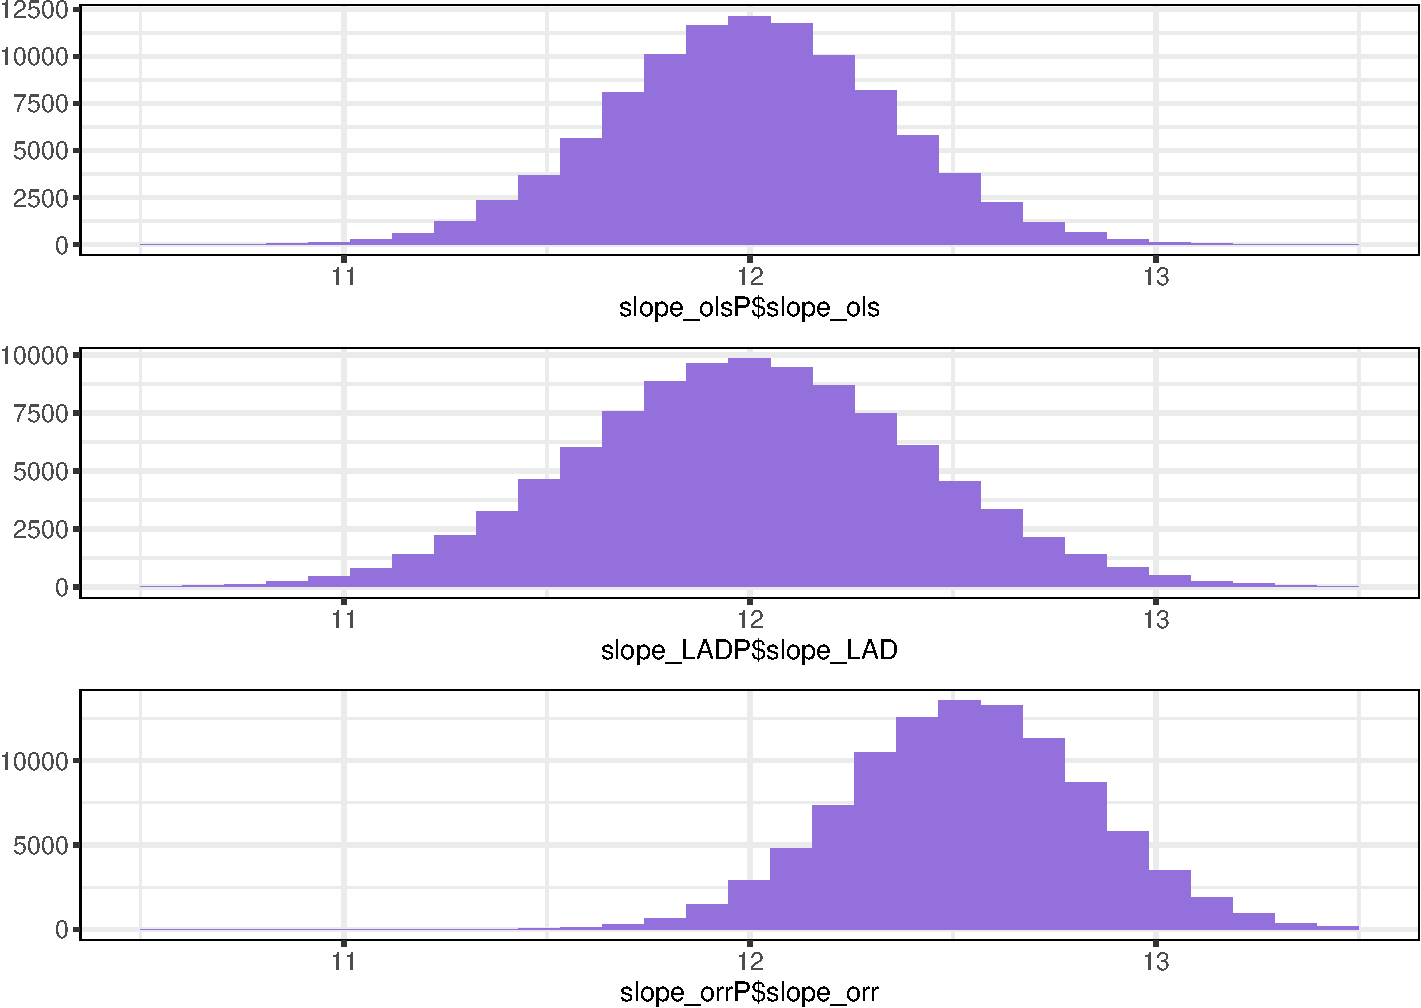
\includegraphics{../graphs/unnamed-chunk-29-1.pdf}
\end{column}
\end{columns}

\end{frame}

\begin{frame}[fragile]{Can we plot the conditional effects too?}
\protect\hypertarget{can-we-plot-the-conditional-effects-too}{}

\begin{columns}[T]
\begin{column}{0.5\textwidth}
\tiny

\begin{Shaded}
\begin{Highlighting}[]
\KeywordTok{glm}\NormalTok{(mpg }\OperatorTok{\textasciitilde{}}\StringTok{ }\NormalTok{hp}\OperatorTok{*}\NormalTok{wt}\OperatorTok{*}\KeywordTok{as.factor}\NormalTok{(cyl), }\DataTypeTok{data =}\NormalTok{ mtcars) }\OperatorTok{\%\textgreater{}\%}
\StringTok{  }\KeywordTok{cplot}\NormalTok{(}\DataTypeTok{x =} \StringTok{"cyl"}\NormalTok{, }\DataTypeTok{draw =}\NormalTok{ F) }\OperatorTok{\%\textgreater{}\%}
\StringTok{  }\KeywordTok{ggplot}\NormalTok{( }\KeywordTok{aes}\NormalTok{(}\DataTypeTok{x =} \KeywordTok{reorder}\NormalTok{(xvals, yvals),}
                      \DataTypeTok{y =}\NormalTok{ yvals, }\DataTypeTok{ymin =}\NormalTok{ lower, }\DataTypeTok{ymax =}\NormalTok{ upper))}\OperatorTok{+}
\StringTok{                      }\KeywordTok{geom\_hline}\NormalTok{(}\DataTypeTok{yintercept =} \DecValTok{0}\NormalTok{, }\DataTypeTok{color =} \StringTok{"gray80"}\NormalTok{) }\OperatorTok{+}
\StringTok{                      }\KeywordTok{geom\_pointrange}\NormalTok{() }\OperatorTok{+}\StringTok{ }\KeywordTok{coord\_flip}\NormalTok{() }\OperatorTok{+}
\StringTok{    }\KeywordTok{labs}\NormalTok{(}\DataTypeTok{x =} \StringTok{"Number of cylinders"}\NormalTok{, }\DataTypeTok{y =} \StringTok{"Conditional Effect"}\NormalTok{) }\OperatorTok{+}
\StringTok{    }\KeywordTok{theme\_luis}\NormalTok{()}
\end{Highlighting}
\end{Shaded}
\end{column}

\begin{column}{0.5\textwidth}

\includegraphics{../graphs/unnamed-chunk-31-1.pdf}
\end{column}
\end{columns}

\end{frame}

\begin{frame}{Oddities of interactions in linear regressions}
\protect\hypertarget{oddities-of-interactions-in-linear-regressions}{}

\begin{itemize}
\tightlist
\item
  At the beginning I said, keep the interaction that is significant,
  but\footnote<.->{Bruin, ``Deciphering Interactions in Logistic
    Regression,'' \emph{Introduction to SAS. UCLA: Statistical
    Consulting Group.}; Vanhove, 2019, ``Interactions in Logistic
    Regression Models,'' (2019).}

  \begin{itemize}
  \tightlist
  \item
    In the conversion to probabilities (AME) the interaction may not be
    significant anymore, or worse
  \item
    The interaction may be significant in the AME, but not in the
    original model
  \end{itemize}
\end{itemize}

\end{frame}

\begin{frame}[fragile]{In OpenMX, maximum likelihood}
\protect\hypertarget{in-openmx-maximum-likelihood}{}

\begin{columns}[T]
\begin{column}{0.4\textwidth}
\tiny

\begin{Shaded}
\begin{Highlighting}[]
\KeywordTok{library}\NormalTok{(umx)}

\NormalTok{model \textless{}{-}}\StringTok{ "}
\StringTok{  mpg \textasciitilde{} a*hp + b*wt }
\StringTok{  moderation := a*b}
\StringTok{"}

\KeywordTok{umxRAM}\NormalTok{(model, }\DataTypeTok{data =}\NormalTok{ mtcars, }\DataTypeTok{tryHard=}\StringTok{"ordinal"}\NormalTok{, }
       \DataTypeTok{silent =}\NormalTok{ T)}
\end{Highlighting}
\end{Shaded}
\end{column}

\begin{column}{0.6\textwidth}
\tiny

\begin{longtable}[]{@{}llrrl@{}}
\toprule
& name & Estimate & SE & type\tabularnewline
\midrule
\endhead
5 & hp\_with\_wt & 42.812 & 13.758 & Manifest Cov\tabularnewline
1 & a & -0.032 & 0.009 & Manifest path\tabularnewline
2 & b & -3.878 & 0.602 & Manifest path\tabularnewline
7 & one\_to\_mpg & 37.227 & 1.522 & Mean\tabularnewline
8 & one\_to\_hp & 146.687 & 11.929 & Mean\tabularnewline
9 & one\_to\_wt & 3.217 & 0.170 & Mean\tabularnewline
3 & mpg\_with\_mpg & 6.095 & 1.524 & Residual\tabularnewline
4 & hp\_with\_hp & 4553.963 & 1138.504 & Residual\tabularnewline
6 & wt\_with\_wt & 0.927 & 0.232 & Residual\tabularnewline
\bottomrule
\end{longtable}

Model Fit: Chi2(0) = 0, p = 1.000; CFI = 1; TLI = 1; RMSEA = 0
Algebra'moderation' = 0.123CI95{[}0.074, 0.173{]}. p-value \textless{}
0.001
\end{column}
\end{columns}

\end{frame}

\begin{frame}{Conclusion}
\protect\hypertarget{conclusion}{}

\begin{itemize}
\tightlist
\item
  We started reviewing multiple regression
\item
  Then discussed the syntax and interpretation of parameters when an
  interaction term is included
\item
  Finally, we discussed how to extract the marginal effects of the
  interaction term
\item
  Luckly the package margins() makes this extremely simple.
\end{itemize}

\end{frame}

\begin{frame}{Acknowledgements}
\protect\hypertarget{acknowledgements}{}

\begin{columns}[T]
\begin{column}{0.5\textwidth}
\begin{block}{Team}

\begin{itemize}
\tightlist
\item
  Charles Gardner (2015)
\item
  Brad Verhulst (2013)
\item
  Joshua Pritkin.
\item
  Rob Kirkpatrick.
\end{itemize}

\vspace{3mm}

\begin{itemize}
\item
  Michael C Neale.
\item
  NIH grant no R01 DA049867 and 5T32MH-020030
\end{itemize}

\end{block}
\end{column}

\begin{column}{0.5\textwidth}
\begin{block}{Contact}

\begin{center}
\includegraphics[width=0.8\linewidth]{../graphs/qr-twitter-1} \end{center}

\end{block}
\end{column}
\end{columns}

\appendix

\end{frame}

\begin{frame}[standout]{}
\protect\hypertarget{section-2}{}

\begin{itemize}
\tightlist
\item
  Thank you
\end{itemize}

\end{frame}

\end{document}
